\chapter{DevOps و نقش آن در فرایند تکامل نرم‌افزار}

\section{3.1 مقدمه و تعریف DevOps}
\label{sec:ch3-Definition}
\section{مقدمه و تعریف DevOps}
\subsection*{3.1 مقدمه و تعریف DevOps}
DevOps یک فرهنگ، فلسفه و مجموعه‌ای از روش‌ها و ابزارها است که هدف اصلی آن، یکپارچه‌سازی و خودکارسازی فرآیندهای بین تیم‌های توسعه نرم‌افزار (Development) و عملیات فناوری اطلاعات (Operations) است. در مدل سنتی، این دو تیم جدا از هم عمل می‌کردند که منجر به کندی، خطاهای بیشتر و هماهنگی دشوار می‌شد. ظهور DevOps پاسخی به این چالش‌ها بود تا با ایجاد همکاری و مسئولیت مشترک، شکاف بین ساخت نرم‌افزار و اجرای پایدار آن را از بین ببرد. در نهایت، DevOps به سازمان‌ها این توانایی را می‌دهد که نرم‌افزارها را سریع‌تر، قابل‌اطمینان‌تر و با کیفیت بالاتر در اختیار کاربران قرار دهند.

\begin{figure}[h]
\centering
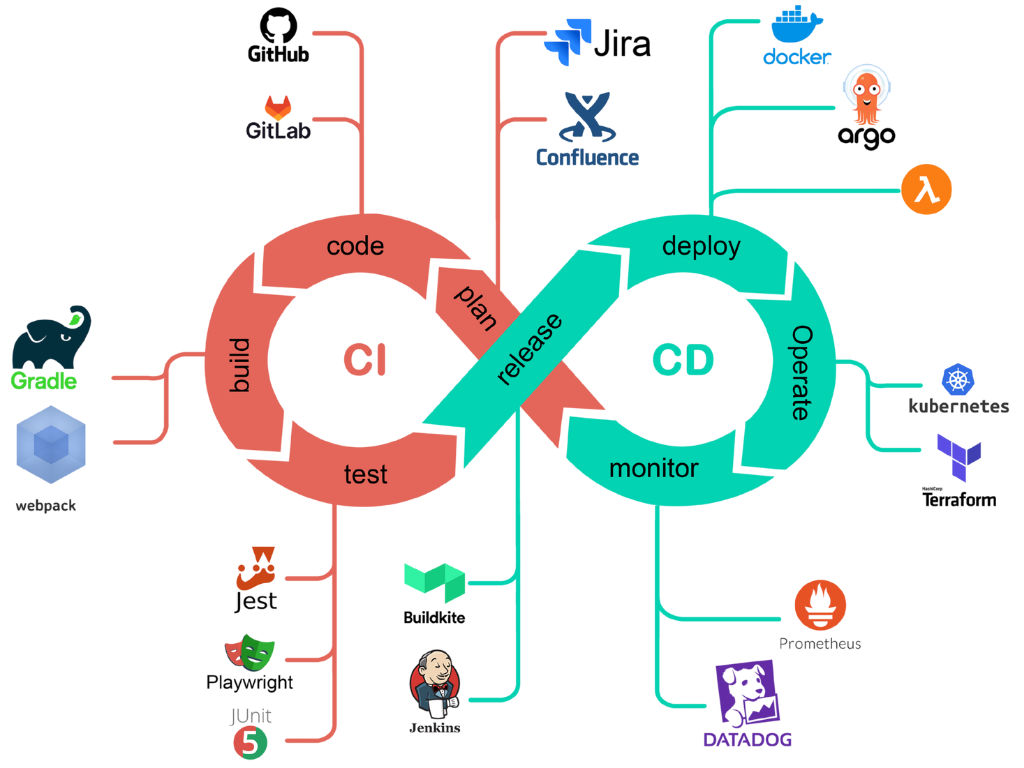
\includegraphics[width=0.8\textwidth]{image9.png}
\caption{DevOps life-cycle and tools}
\label{fig:DevOps life-cycle and tools}
\end{figure}



\section{3.2 فلسفه DevOps و ارتباط آن با Agile}
\label{sec:ch3-DevOpsVSAgile}
\section{فلسفه DevOps و ارتباط آن با Agile}
فلسفه DevOps بر پایه اصولی استوار است که فرهنگ همکاری، خودکارسازی و بهبود مستمر را ترویج می‌دهد. این فلسفه را می‌توان در "حلقه بی‌پایان" عملیات DevOps (که شامل مراحل برنامه‌ریزی، توسعه، استقرار و نظارت است) و همچنین در "سه راهی" معروف آن (جریان (Flow)، بازخورد (Feedback) و یادگیری مستمر (Continuous Learning)) خلاصه کرد.

ارتباط DevOps با متدولوژی Agile بسیار عمیق است. Agile بر انعطاف‌پذیری، تحویل تدریجی و پاسخگویی به تغییرات در طول فرآیند توسعه تأکید دارد. DevOps این فلسفه را گسترش می‌دهد و آن را به فرآیند استقرار و عملیات پس از توسعه تسری می‌بخشد. در حقیقت، DevOps مکمل Agile است؛ در حالی که Agile سرعت و کیفیت توسعه را افزایش می‌دهد، DevOps تضمین می‌کند که این تغییرات سریع می‌توانند به صورت ایمن و پایدار در محیط تولید مستقر شوند. بنابراین، می‌توان DevOps را به عنوان ادامه طبیعی و ضروری جنبش Agile در نظر گرفت که تمرکز آن بر روی کل چرخه عمر نرم‌افزار است.



\section{3.3 چرخه عمر DevOps}
\label{sec:ch3-LifeCicle}
\section{چرخه عمر DevOps}
\subsection*{3.3 چرخه عمر DevOps}
چرخه عمر DevOps یک فرآیند تکراری و مستمر است که مراحل مختلفی از ایده تا تحویل نرم‌افزار و نظارت بر آن را در بر می‌گیرد. این چرخه با استفاده از ابزارهای خودکار به هم پیوسته، جریان ارزش را سریع و کارآمد می‌کند.

\begin{itemize}
    \item \textbf{برنامه‌ریزی (Plan)} \\
    در این فاز اولیه، اهداف پروژه تعریف، وظایف زمان‌بندی و پیشرفت کار رهگیری می‌شود. این مرحله تضمین می‌کند که همه اعضای تیم از اهداف کسب‌وکار و برنامه‌های فنی آگاه هستند. \\
    \textbf{ابزارها:} از ابزارهایی مانند Jira برای ردیابی Issues و مدیریت پروژه و Confluence برای مستندسازی و همکاری استفاده می‌شود.

    \item \textbf{توسعه (Code)} \\
    توسعه‌دهندگان در این مرحله نرم‌افزار را می‌نویسند. برای اطمینان از سازگاری و قابلیت تکرار محیط‌های توسعه، از ابزارهای خاصی استفاده می‌شود. \\
    \textbf{ابزارها:} Docker برای بسته‌بندی نرم‌افزار در کانتینرهای سبک و قابل حمل، Kubernetes برای مدیریت و خودکارسازی این کانتینرها، و Ansible \& Puppet برای مدیریت پیکربندی و خودکارسازی زیرساخت به کار می‌روند.

    \item \textbf{یکپارچه‌سازی مستمر (\lr{Continuous Integration})} \\
    این تمرین شامل ادغام مکرر کد نوشته‌شده توسط تمام توسعه‌دهندگان به یک ریپازیتوری مشترک است. پس از هر ادغام، فرآیندهای ساخت و تست به طور خودکار اجرا می‌شوند تا خطاها در اسرع وقت شناسایی شوند. CI تضمین می‌کند که کدها به طور مداوم با یکدیگر یکپارچه شده و از بروز تعارضات بزرگ در آینده جلوگیری می‌کند.

    \item \textbf{تحویل مستمر (\lr{Continuous Delivery})} \\
    CD گام بعدی پس از CI است. این تمرین تضمین می‌کند که پس از هر ادغام موفقیت‌آمیز کد، می‌توان نرم‌افزار را در هر لحظه و با کمترین تلاش به صورت دستی در محیط تولید منتشر کرد. در تحویل مستمر، فرآیند استقرار تا مرحله نهایی خودکار است، اما انتشار نهایی در محیط تولید به صورت دستی و با تأیید یک انسان انجام می‌شود.

    \item \textbf{استقرار مستمر (\lr{Continuous Deployment})} \\
    این پیشرفته‌ترین مرحله است که در آن، هر تغییری که از تست‌ها در مراحل CI/CD موفقیت‌آمیز عبور کند، به طور خودکار در محیط تولید مستقر می‌شود. در این مدل، هیچ مداخله دستی در فرآیند استقرار وجود ندارد و انتشار نرم‌افزار به یک رویداد عادی و روزمره تبدیل می‌شود. این امر سرعت ارائه ارزش به کاربر نهایی را به حداکثر می‌رساند. \\
    \textbf{ابزارهای CI/CD:} از ابزارهایی مانند Jenkins, GitHub Actions/GitLab CI/CD و CircleCI برای خودکارسازی کامل خط لوله از یکپارچه‌سازی تا استقرار استفاده می‌شود.

    \item \textbf{نظارت و بازخورد (\lr{Monitoring \& Feedback})} \\
    پس از استقرار نرم‌افزار در محیط تولید، عملکرد آن تحت نظارت دقیق قرار می‌گیرد تا از پایداری و سلامت سرویس اطمینان حاصل شود. داده‌های مربوط به عملکرد برنامه، زیرساخت و تجربه کاربر جمع‌آوری و تجزیه و تحلیل می‌شوند. این داده‌ها به صورت یک حلقه بازخورد (Feedback Loop) به تیم‌های توسعه و برنامه‌ریزی بازمی‌گردند تا برای بهبود مستمر محصول و رفع مشکلات در چرخه‌های بعدی مورد استفاده قرار گیرند. \\
    \textbf{ابزارها:} Grafana برای تجسم متریک‌ها، Elastic Stack برای مدیریت و تحلیل لاگ‌ها، Prometheus برای مانیتورینگ و هشدار و Sentry برای ردیابی خطاها در لحظه استفاده می‌شوند.
\end{itemize}


\section{پیشنهادات برای کارهای آینده}
\label{sec:ch4-future}
بر اساس نتایج و محدودیت‌های شناسایی شده، پیشنهادات زیر برای کارهای آینده ارائه می‌شود:

\subsection{بهبودهای کوتاه‌مدت}
\begin{enumerate}
    \item بهینه‌سازی کد برای کاهش مصرف حافظه
    \item افزودن قابلیت‌های جدید به سیستم
    \item بهبود رابط کاربری
\end{enumerate}

\subsection{پیشنهادات برای تحقیقات آینده}
\begin{itemize}
    \item بررسی استفاده از روش‌های یادگیری عمیق
    \item توسعه نسخه توزیع شده از سیستم
    \item ارزیابی روی مجموعه داده‌های بزرگ‌تر
    \item مطالعه کاربردهای جدید در حوزه‌های دیگر
\end{itemize}

\subsection{کاربردهای بالقوه}
این کار می‌تواند در زمینه‌های زیر کاربرد داشته باشد:
\begin{itemize}
    \item صنعت و تولید
    \item آموزش و پژوهش
    \item خدمات و تجارت الکترونیک
\end{itemize}




\section{فرهنگ و سازمان‌دهی در DevOps}
\label{sec:ch3-5-culture}
بر اساس نتایج و محدودیت‌های شناسایی شده، پیشنهادات زیر برای کارهای آینده ارائه می‌شود:

\subsection{بهبودهای کوتاه‌مدت}
\begin{enumerate}
    \item بهینه‌سازی کد برای کاهش مصرف حافظه
    \item افزودن قابلیت‌های جدید به سیستم
    \item بهبود رابط کاربری
\end{enumerate}

\subsection{پیشنهادات برای تحقیقات آینده}
\begin{itemize}
    \item بررسی استفاده از روش‌های یادگیری عمیق
    \item توسعه نسخه توزیع شده از سیستم
    \item ارزیابی روی مجموعه داده‌های بزرگ‌تر
    \item مطالعه کاربردهای جدید در حوزه‌های دیگر
\end{itemize}

\subsection{کاربردهای بالقوه}
این کار می‌تواند در زمینه‌های زیر کاربرد داشته باشد:
\begin{itemize}
    \item صنعت و تولید
    \item آموزش و پژوهش
    \item خدمات و تجارت الکترونیک
\end{itemize}




\section{مزایای DevOps در تکامل نرم‌افزار}
\label{sec:ch3-6-benefits}
% chapters/chapter3/section6.tex
% این فایل را فایل اصلی فصل با \input وارد می‌کند، پس نباید \section یا \subsection عنوان اصلی داشته باشد.

مهم‌ترین مزایای به‌کارگیری \lr{DevOps} در فرایند توسعه و تکامل نرم‌افزار عبارت‌اند از:
\begin{itemize}
    \item افزایش سرعت تحویل نرم‌افزار
    \item بهبود پایداری و اطمینان در استقرارها
    \item ارتقای کیفیت محصول
    \item افزایش بهره‌وری و هماهنگی تیم‌ها
    \item توانایی پاسخ سریع به تغییرات بازار و نیازهای کاربران
\end{itemize}
همان‌طور که در \cite{Jha2023} نیز اشاره شده است، این مزایا زمانی به‌طور کامل به دست می‌آیند که فرهنگ همکاری میان تیم‌های توسعه و عملیات که در بخش \ref{subsec:ch3-5-collaboration} توضیح داده شد، در سازمان نهادینه شده باشد.

\subsubsection*{افزایش سرعت تحویل نرم‌افزار}
\lr{DevOps} موجب می‌شود چرخه‌ی توسعه از ایده تا تحویل نهایی کوتاه‌تر شود. با خودکارسازی مراحلی مانند ساخت، تست و استقرار، تیم‌ها می‌توانند در بازه‌های زمانی بسیار کوتاه نسخه‌های جدید ارائه دهند. به‌عنوان نمونه، شرکت \lr{Amazon} روزانه هزاران استقرار جدید در زیرساخت خود انجام می‌دهد. این حجم از به‌روزرسانی تنها به لطف استفاده از خطوط خودکار \lr{CI/CD} ممکن است.

\subsubsection*{بهبود پایداری و اطمینان در استقرارها}
در روش‌های سنتی، استقرار نرم‌افزار اغلب با اضطراب و خطا همراه بود، زیرا تغییرات به‌صورت گسترده و یک‌باره اعمال می‌شد. \lr{DevOps} این مشکل را با اعمال تغییرات کوچک و مکرر حل کرده است. نمونه‌ی شناخته‌شده، تجربهٔ \lr{Etsy} است که پس از خودکارسازی استقرارها، توانست بدون توقف سرویس، استقرارهای متعدد روزانه انجام دهد.

\subsubsection*{ارتقای کیفیت محصول}
تست‌های خودکار و مانیتورینگ مستمر از ارکان \lr{DevOps} هستند و کمک می‌کنند خطاها در مراحل ابتدایی شناسایی و اصلاح شوند. شرکت‌هایی مانند \lr{Google} با تکیه بر پایش مداوم، نرخ خرابی را کاهش داده‌اند.

\subsubsection*{افزایش بهره‌وری و هماهنگی تیم‌ها}
\lr{DevOps} باعث می‌شود تیم‌های توسعه، عملیات، آزمون و حتی امنیت در یک چرخه‌ی واحد کار کنند و کارهای دستی و تکراری حذف شود.

\subsubsection*{پاسخ سریع به تغییرات بازار و نیازهای کاربران}
در محیط‌های پویا، چرخه‌ی بازخورد سریع که در \cite{Jha2023} بر آن تأکید شده، امکان انتشار و بازگردانی سریع ویژگی‌ها را فراهم می‌کند.


\section{مطالعه‌ی موردی}
\label{sec:ch3-7-case-study}
% chapters/chapter3/section7.tex
% این فایل را فایل اصلی فصل با \input وارد می‌کند، پس نباید \section یا \subsection داشته باشد.

شرکت \lr{Netflix} با میلیون‌ها کاربر در سراسر جهان، یکی از پیشگامان در به‌کارگیری رویکرد \lr{DevOps} است. مقیاس بسیار بزرگ سامانه و نیاز به ارائهٔ مداوم محتوا، این شرکت را بر آن داشت تا از شیوه‌های سنتی توسعه فاصله بگیرد و معماری‌ای پویا و مبتنی بر خودکارسازی ایجاد کند. همان‌گونه که در پژوهش \cite{Jha2023} نیز تأکید شده، موفقیت در مقیاس گسترده تنها زمانی ممکن است که فرهنگ سازمانی، ابزارها و فرآیندها هم‌زمان دگرگون شوند.

\subsubsection*{چالش‌های اولیه}

در سال‌های ابتدایی فعالیت، \lr{Netflix} با چند چالش اساسی روبه‌رو بود:
\begin{itemize}
    \item استقرارهای نرم‌افزاری به‌صورت دستی انجام می‌شد و احتمال خطاهای انسانی بالا بود.
    \item هرگونه تغییر کوچک در سیستم می‌توانست موجب اختلال در پخش محتوا شود.
    \item سرورها در مراکز دادهٔ داخلی نگهداری می‌شدند و مقیاس‌پذیری آن‌ها محدود بود.
\end{itemize}

این چالش‌ها سبب شدند که \lr{Netflix} در سال ۲۰۰۸ تصمیم بگیرد به زیرساخت ابری مهاجرت کند و هم‌زمان فلسفهٔ \lr{DevOps} را در سازمان پیاده‌سازی کند. این تصمیم، نقطهٔ عطفی در مسیر تکامل فنی و فرهنگی شرکت بود.

\subsubsection*{معماری و ابزارهای مورد استفاده}

برای تحقق اصول \lr{DevOps}، \lr{Netflix} مجموعه‌ای از ابزارها و فرآیندهای خودکار را توسعه داد. برخی از مهم‌ترین آن‌ها عبارت‌اند از:
\begin{itemize}
    \item \textbf{\lr{Spinnaker}:} سیستم متن‌باز ویژهٔ \lr{Netflix} برای خودکارسازی خط لوله‌های \lr{CI/CD}. این ابزار امکان استقرار مکرر، سریع و بدون وقفهٔ سرویس‌ها را فراهم می‌کند.
    \item \textbf{\lr{Chaos Monkey}:} ابزاری برای آزمایش پایداری سیستم از طریق ایجاد خطاهای تصادفی در سرورها؛ هدف آن ارزیابی مقاومت سامانه در برابر شکست است.
    \item \textbf{\lr{Atlas}} و \textbf{\lr{Vector}:} ابزارهای پایش و تحلیل عملکرد سرویس‌ها که داده‌ها را به‌صورت لحظه‌ای جمع‌آوری و بررسی می‌کنند.
\end{itemize}

با این زیرساخت‌ها، \lr{Netflix} قادر است روزانه صدها استقرار جدید انجام دهد، بدون آن‌که کاربران هیچ‌گونه اختلالی در سرویس احساس کنند.

\subsubsection*{فرهنگ سازمانی \lr{DevOps} در \lr{Netflix}}

مطابق با دیدگاه مطرح‌شده در \cite{Jha2023}، یکی از عوامل کلیدی موفقیت \lr{DevOps} در \lr{Netflix}، نهادینه‌سازی آن در فرهنگ سازمانی است. اصول فرهنگی مهم در این شرکت شامل موارد زیر است:
\begin{itemize}
    \item \textbf{اعتماد به تیم‌ها:} هر تیم مسئول استقرار و نگهداری سرویس‌های خود است.
    \item \textbf{آزادی همراه با مسئولیت:} توسعه‌دهندگان در انتخاب ابزار و روش‌ها آزادی کامل دارند، اما مسئولیت عملکرد سرویس نیز با خود آنان است.
    \item \textbf{بازخورد سریع:} داده‌های واقعی کاربران به‌صورت لحظه‌ای تحلیل می‌شود و تصمیم‌گیری‌ها بر پایهٔ شواهد انجام می‌گیرد.
\end{itemize}

\subsubsection*{نتایج پیاده‌سازی}

اجرای اصول \lr{DevOps} در \lr{Netflix} منجر به بهبود چشمگیر در جنبه‌های مختلف توسعه و بهره‌برداری از سامانه شده است:
\begin{itemize}
    \item کاهش محسوس خطاهای استقرار،
    \item افزایش سرعت ارائهٔ قابلیت‌های جدید،
    \item مقیاس‌پذیری بسیار بالا در پاسخ به رشد کاربران،
    \item ارتقای تجربهٔ کاربری و کاهش زمان قطعی سرویس.
\end{itemize}

به‌عنوان نمونه، در زمان اوج مصرف، سامانه‌های \lr{Netflix} قادرند میلیون‌ها درخواست هم‌زمان را بدون افت کیفیت پاسخ دهند؛ قابلیتی که بدون زیرساخت خودکار و فرهنگ همکاری \lr{DevOps} امکان‌پذیر نبود.


\section{چالش‌های استقرار DevOps}
\label{sec:ch3-8-challenges}
% chapters/chapter3/section8.tex
% این فایل را فایل اصلی فصل با \input وارد می‌کند، پس نباید \section یا \subsection داشته باشد.

هرچند \lr{DevOps} در سال‌های اخیر به‌عنوان یکی از مؤثرترین رویکردها در توسعهٔ نرم‌افزار شناخته شده است، اما پیاده‌سازی موفق آن کار ساده‌ای نیست. همان‌گونه که در پژوهش \cite{Jha2023} نیز اشاره شده، سازمان‌ها در مسیر استقرار \lr{DevOps} با موانع فنی و فرهنگی متعددی روبه‌رو می‌شوند که در صورت مدیریت‌نشدن صحیح، می‌توانند موجب کندی یا حتی شکست کل فرآیند شوند. در ادامه، مهم‌ترین چالش‌های پیاده‌سازی این رویکرد بررسی می‌شود.

\subsubsection*{مسائل امنیتی و حفظ اعتماد}

با خودکار شدن فرآیندها و افزایش سرعت استقرار، امنیت به یکی از دغدغه‌های اصلی در محیط‌های \lr{DevOps} تبدیل شده است. در روش‌های سنتی، بررسی‌های امنیتی معمولاً در انتهای چرخهٔ توسعه انجام می‌شد، اما در \lr{DevOps} انتشارهای سریع و مکرر ممکن است سبب نادیده‌گرفتن برخی کنترل‌های حیاتی شود. برای نمونه، زمانی که تیم توسعه به‌صورت روزانه کد جدید را با شاخهٔ اصلی ادغام می‌کند، یک آسیب‌پذیری کوچک می‌تواند بلافاصله وارد محیط تولید شود.
برای رفع این مشکل، رویکرد \lr{DevSecOps} پیشنهاد می‌شود که در آن، امنیت از مراحل اولیهٔ توسعه در چرخهٔ عمر نرم‌افزار ادغام می‌شود. همچنین کنترل دسترسی، مدیریت کلیدها و محافظت از داده‌های حساس از مسئولیت‌های مهمی هستند که نیاز به نظارت مداوم دارند.

\subsubsection*{پیچیدگی زیرساخت و وابستگی به ابزارها}

یکی دیگر از چالش‌های جدی، افزایش پیچیدگی فنی در اثر استفاده از ابزارهای متنوع است. سازمان‌ها برای پیاده‌سازی \lr{DevOps} اغلب از ترکیب ابزارهایی چون \lr{Docker}، \lr{Kubernetes}، \lr{Jenkins} و \lr{Terraform} استفاده می‌کنند. هرچند این ابزارها قدرت و انعطاف بالایی دارند، اما برای تیم‌هایی که تجربهٔ کافی ندارند، می‌توانند موجب سردرگمی و کاهش بهره‌وری شوند.
مطالعهٔ \cite{Jha2023} نشان می‌دهد تمرکز بیش از حد بر ابزارها ممکن است هدف اصلی \lr{DevOps} یعنی همکاری مؤثر و تحویل سریع ارزش به مشتری را تحت‌الشعاع قرار دهد. مستندسازی دقیق، آموزش منظم و طراحی زیرساخت ساده و پایدار از مهم‌ترین راهکارهای مقابله با این چالش هستند.

\subsubsection*{مقاومت فرهنگی و تغییر در شیوهٔ کار}

مهم‌ترین مانع در مسیر اجرای \lr{DevOps}، چالش فرهنگی درون سازمان است. برخلاف تصور رایج، \lr{DevOps} صرفاً تغییر در ابزارها نیست، بلکه تحولی در نگرش، ساختار و مسئولیت‌پذیری اعضاست. در مدل سنتی، تیم‌های توسعه و عملیات معمولاً به‌صورت مجزا عمل می‌کردند و هرکدام تنها بخشی از مسئولیت را بر عهده داشتند؛ اما در \lr{DevOps} مرزها از میان برداشته می‌شوند و موفقیت کل محصول، مسئولیتی جمعی است.
در بسیاری از سازمان‌ها، این تغییر ذهنیت با مقاومت مواجه می‌شود — به‌ویژه در ساختارهای سلسله‌مراتبی که عادت به تفکیک نقش‌ها دارند. تجربهٔ گزارش‌شده در \cite{Jha2023} نشان می‌دهد آموزش مستمر، شفاف‌سازی اهداف و مشارکت فعال کارکنان در تصمیم‌گیری، از مؤثرترین راهکارها برای غلبه بر این مقاومت فرهنگی است.

در مجموع، استقرار موفق \lr{DevOps} مستلزم آمادگی فنی و فرهنگی توأمان است. بی‌توجهی به یکی از این ابعاد می‌تواند موجب کندی در تحول سازمانی و کاهش اثربخشی کل چرخهٔ توسعه شود.



\section{جمع‌بندی فصل}
\label{sec:ch3-9-summary}
% chapters/chapter3/section9.tex
% این فایل را فایل اصلی فصل با \input وارد می‌کند، پس نباید \section داشته باشد.

در این فصل نشان داده شد که \lr{DevOps} فراتر از مجموعه‌ای از ابزارها یا روش‌های فنی است و در واقع یک تغییر بنیادی در فرهنگ و نگرش سازمانی به شمار می‌آید. بر اساس پژوهش \cite{Jha2023}، موفقیت در اجرای \lr{DevOps} زمانی حاصل می‌شود که سازمان‌ها بر سه محور کلیدی تمرکز کنند: \textit{همکاری مستمر، مسئولیت‌پذیری مشترک و بهبود پیوسته}. در چنین بستری، مرز میان تیم‌های توسعه و عملیات از میان برداشته می‌شود و کل سازمان به یک واحد منسجم در راستای تحویل ارزش به کاربر تبدیل می‌گردد.

رویکرد \lr{DevOps} با اتکا به خودکارسازی، زیرساخت به‌عنوان کد (\lr{Infrastructure as Code}) و چرخه‌های یکپارچهٔ \lr{CI/CD}، توانسته است فاصله میان تولید نرم‌افزار و استقرار آن را به‌طور چشمگیری کاهش دهد. نتیجهٔ این تحول، تولید نرم‌افزارهایی با کیفیت بالاتر، قابلیت اطمینان بیشتر و سرعت انتشار بالاتر است. ابزارهایی مانند \lr{Jenkins}، \lr{Docker} و \lr{Kubernetes} ستون‌های فنی این رویکرد را تشکیل می‌دهند و زمینه را برای پیاده‌سازی پایدار و مقیاس‌پذیر فرآیندها فراهم می‌کنند.

نمونه‌های موفقی همچون \lr{Netflix} و \lr{Amazon} نشان داده‌اند که اجرای اصول \lr{DevOps} نه‌تنها موجب افزایش چابکی و مقیاس‌پذیری می‌شود، بلکه توانایی سازمان در پاسخ‌گویی به تغییرات بازار و نیاز کاربران را نیز ارتقا می‌دهد. با این حال، همان‌گونه که در \cite{Jha2023} تأکید شده، استقرار \lr{DevOps} بدون آمادگی فرهنگی و آموزشی کافی می‌تواند با چالش‌هایی چون پیچیدگی زیرساخت، ضعف در امنیت و مقاومت کارکنان روبه‌رو شود.

در نهایت می‌توان \lr{DevOps} را پلی میان فرهنگ \lr{Agile} و عملیات مدرن دانست؛ پلی که با تقویت ارتباط میان فناوری، فرآیند و فرهنگ همکاری، مسیر تحول دیجیتال را هموار می‌سازد. سازمان‌هایی که بتوانند میان این سه بُعد تعادل برقرار کنند، نه‌تنها در توسعهٔ نرم‌افزار بلکه در کل چرخهٔ عمر نوآوری و ارزش‌آفرینی خود به موفقیت پایدار دست خواهند یافت.

